\documentclass[a4paper,12pt]{report}
\usepackage[utf8]{inputenc}


\usepackage{tikz}
\usetikzlibrary{calc}
\usepackage{subcaption}

\begin{document}

\thispagestyle{empty}

\begin{figure}[h!]
		\centering
		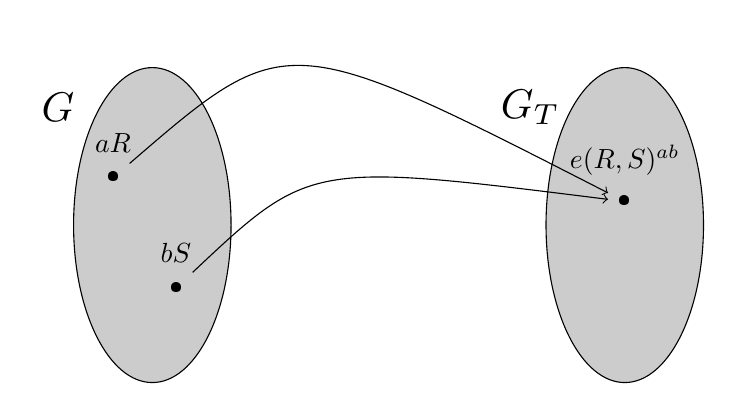
\begin{tikzpicture}
		
		\node[scale=1.5] at (-1.2,2.5) {$G$};
		\filldraw[black!20!white, draw=black] (0,1) ellipse (1cm and 2cm);
		\node[label={$aR$},scale=1] (1) at (-0.5,1.6) {\textbullet};
		\node[label={$bS$},scale=1] (2) at (0.3,0.2) {\textbullet};
		
		\node[scale=1.5] at (4.8,2.5) {$G_T$};
		\filldraw[black!20!white, draw=black] (6,1) ellipse (1cm and 2cm);
		\node[label={$e(R,S)^{ab}$},scale=1] (3) at (6,1.3) {\textbullet};
		
		\draw [->] (1) .. controls (1.7,3.5) .. (3) ;
		\draw [->] (2) .. controls (2,1.8) .. (3) ;
	
		\end{tikzpicture}
		\caption{A symmetric bilinear pairing.}
		\label{fig:pairing}
	\end{figure}

\end{document}
